\section{Introduction}
Chapter \ref{ch2} has shown how random waves can be usually treated as a 
sum of linear waves with random phases. Chapter \ref{ch_sourceterms} presented how it evolves under the influence of weak non-linearities 
as described by a wave action equation. Non-linearities actually become stronger in shallow water when the waves are less dispersive ($kD << 1$), 
and we have to reconsider the non-linear effects. In chapter \ref{ch1b} we have introduced the two small parameters 
$\varepsilon=ka$ and $\delta=a/D$. The nonlinear effects that we will discuss here occur when the parameter $U_r = \delta^3/\varepsilon^2= a/k^2 D^3$ is 
of order 1. This parameter was introduced by \cite{Ursell1953}. The regime $U_r  \ll 1$ corresponds to the weak nonlinearity already 
discussed in chapter  \ref{ch_sourceterms}. 

The stronger non-linearity that occurs for $U_r=O(1)$ correspond to a near-resonance at second order, i.e. $k_3 \simeq k_1 + k_2$ and 
 $f_3 = f_1 \pm f_2$, with the plus sign giving super-harmonics of higher frequency, and the minus sign giving sub-harmonics of very low frequency 
 or infragravity waves. These interactions can also be seen as a non-linear wave scattering by the bottom topography with $\kb_3 =  \kb_1 + \kb_2 + \kb_b$ 
 where $\kb_b$ is the wavenumber of the topography \citep{Liu&Yue1998,Groeneweg&al.2015}. 

Instead of going back to the full Euler equations, several approximations have been proposed to simplify the problem but keep the nonlinearity. 
In  particular, assuming weak dispersion ($kD << 1$) allows to derive a simplified set of equations. 

\section{Boussinesq and KdV equations}
Both the Boussinesq and \citet[][KdV for short]{Korteweg&deVries1895} equations were first derived by \cite{Boussinesq1872} for waves propagating in one direction. We will 
here use the form given by \cite{Peregrine1967}, 
\begin{equation}
    \frac{\partial \zeta}{\partial t}+\sqrt{gD} \left( \frac{\partial \zeta}{\partial x}+\frac{3}{2D} \zeta \frac{\partial \zeta}{\partial x}
    +\frac{D^2}{6} \frac{\partial^3 \zeta}{\partial x^3} \right)=0. \label{eq:KdV}
\end{equation}
This is asymptotically valid for $kD << 1$ and $ka << 1$. For a constant depth $D$, 
solutions to the KdV equation include quasi-periodic recurrent amplitudes 
\citep{Fermi&al.1955} caused by the near resonances $k_3 \simeq k_1 + k_2$  which exist when $kD<< 1$. 

Interestingly, the KdV equation can be solved exactly using the inverse scattering transform, which expresses the solution 
as a superposition of interacting waves trains and solitary waves also known as cnoidal waves or solitons \citep{Osborne&al.1996}. 
Among these cnoidal waves, the classical solitary wave solution is, 
\begin{equation}
    \zeta=\frac{a}{ \cosh^2\left[\sqrt{ 3a / D^3}\left(x-Ct\right)\right]} \label{eq:solitary}
\end{equation}
%%%%%%%%%%%%%%%%%%%%%%%%%%%%%%%%%%%%%%%%%%%%%%%%%%%%%%% figure
\begin{figure}
\centerline{\includegraphics[width=0.8\textwidth]{FIGS_CH_SURF/soliton.pdf}}
%  \vspace{8.0cm}
  \caption{Solitary wave given by eq. (\ref{eq:solitary}) that is a solution of the KdV equation (\ref{eq:KdV}) in the case  $D=10$~m}
\label{soliton}
\end{figure}
%%%%%%%%%%%%%%%%%%%%%%%%%%%%%%%%%%%%%%%%%%%%%% end of figure
with a propagation speed 
\begin{equation}
C=\sqrt{gD} \left(1+\frac{a}{2D}\right). \label{eq:solitary_speed}
\end{equation}
In this solitary wave, the dispersive effect of the finite water depth is exactly 
canceled by the dispersive effect of the finite amplitude, so that the wave propagates without changing form. 
%The KdV equation is also one of the asymptotic limits of the non-linear Schrodinger equation that describes the 
%evolution of narrow-banded waves in deep water 
%\citep{Onorato&al.2002,Osborne&al.2003}.

The two-dimensional version of the KdV equation is the Boussinesq equation with many forms developed to improve on its dispersive properties, i.e. 
trying to extend it beyond $kD \ll 1$ \citep{Nwogu1993,Nadaoka&al.1997}. Other extensions for finite amplitude have been performed by Serre and others
\citep{Lannes&Bonneton2009,Dias&Milewski2010}. Some of these equations have been called fully nonlinear Boussinesq equations but, although they 
are indeed valid for finite amplitude, they are not correct for waves that are nearly breaking and always have round crests, not sharp like a
nearly breaking wave. 

\section{Wave evolution}
As waves shoal, the reduction in group speed $C_g$ comes with an increase in the significant wave height $H_s$, in particular 
for a shore-normal incidence $\theta=0$. 
%%%%%%%%%%%%%%%%%%%%%%%%%%%%%%%%%%%%%%%%%%%%%%%%%%%%%%%%%%%%%%%%%%%%%%%%%%%%%%%%
\begin{figure}[htb]
 \vspace{9pt}
\centerline{\includegraphics[width=0.7\linewidth]{FIGS_CH_SURF/wave_shape_near_breaking.pdf}}
 \caption{Wave profiles computed using the numerical solution method by\cite{Dean1965} and \cite{Dalrymple1974} 
 at 60th order for a 3~m water depth, in the case of deep water waves in (a) and (b) with a period $T=1.5$s ($kD \simeq 5$), and 
 shallow water in  (c) and (d)  with $T=8$s, $kD \simeq 0.45$. The arrows represent orbital velocities. 
 Waves in (a) and (c) are moderately nonlinear ($U_c/C \simeq 0.3$), whereas those in (b) and (d) are nearly 
 breaking ($U_c/C = 0.97$). 
 }
 \label{fig:WAVES}
\end{figure}
%%%%%%%%%%%%%%%%%%%%%%%%%%%%%%%%%%%%%%%%%%%%%%%%%%%%%%%%%%%%%%%%%%%%%%%%%%%%%%%%%
That effect is less severe for oblique propagation as the conserved energy flux is  $C_g H_s^2 \cos \theta
/16$  and $\cos \theta$ increases due to refraction. The wavelength $L$ also reduces as $C=L/T$ slows down and the period remains constant. 
This increase in height $H$ and decrease in wavelength $L$ make the steepness $H/L$ increase. 

\subsection{Waves over a flat bottom}
For a monochromatic wave over a flat bottom, \cite{Miche1944d} studied the shape of the waves of maximum steepness. 
In the frame of reference moving with the phase speed $C$, 
it appears that a singularity develops when the orbital velocity $U_c$ approaches $C$. Figure \ref{fig:WAVES} shows 
the difference between waves with $U_c/C \simeq 0.3$ and $U_c/C = 0.97$. When $U_c/C \simeq 0.3$, waves in deep water look linear 
whereas waves in shallow water look like cnoidal waves. As $U_c/C$ approaches 1, the crest become triangular 
with an angle of 120$^\circ$, as was already found by Stokes for the deep water case.

Hence, using $U_c/C = 1$ as a sufficient condition for wave breaking, 
Miche used an analytic streamfunction expansion from the wave crest to find that the maximum wave height $H_{\max}$ is 
\begin{equation}
 H_{\max}/L \simeq 0.14 \tanh(kD)
\end{equation}
In the limit $kD \rightarrow 0$, this Miche limit is $H_{\max}/D\simeq 0.28 \pi = 0.87$. The deep water limit $kD \rightarrow \infty$ gives the 
previously known $kH/2 = 0.44$.  Miche's approximation is very accurate.  Figure \ref{fig:STREAM}.a shows that it can be improved a little by using  
\begin{equation}
 H_{\max}/L \simeq 0.10 \tanh(kD)+ 0.0298 \tanh^2(kD).
\end{equation}
%%%%%%%%%%%%%%%%%%%%%%%%%%%%%%%%%%%%%%%%%%%%%%%%%%%%%%%%%%%%%%%%%%%%%%%%%%%%%%%
\begin{figure}[htb]
 \vspace{9pt}
\centerline{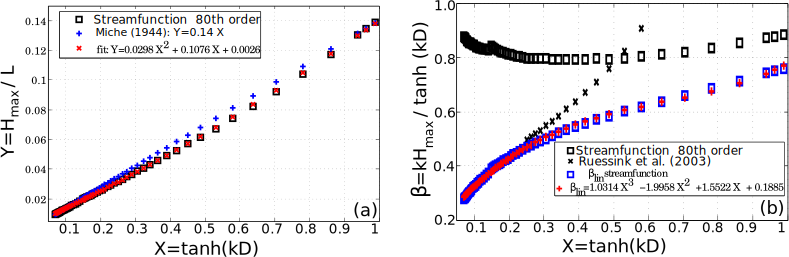
\includegraphics[width=\linewidth]{FIGS_CH_SURF/wave_stream_Hmax.pdf}}
 \caption{Steepness of nearly breaking waves, $Y=H_{max}/L$. The original breaking criterion of Miche (1944) is recalled. 
 A new
 criterion, using a second order polynomial fit for $H/L$ as a function of $X=\tanh(kD)$ is given. 
 The bottom panel shows the alternative
 steepness parameters $\beta$ defined from the wave height, or $\beta_E$ defined from the wave energy. In the case of \cite{Ruessink&al.2003}, his $\gamma$ parameter 
 is interpreted as $H_{max}/D$, and transformed to $\beta_{E}$, using the peak wavenumber $k_p$ to estimate $\bar{k}$ 
 \citep[adapted from ][]{Filipot&al.2010}.}
 \label{fig:STREAM}
\end{figure}
%%%%%%%%%%%%%%%%%%%%%%%%%%%%%%%%%%%%%%%%%%%%%%%%%%%%%%%%%%%%%%%%%%%%%%%%%%%%%%%%%
It should be noted that, so far, we have used $H=2a$ and $E=a^2/2$. In shallow water this does not hold anymore, and the error on the wave 
height can be a factor 3 or more. Even if it is probably less important on a sloping bottom, as we will see below, if one wants to apply a limit on the wave 
height when using wave energy, we can first define
a generalized maximum wave steepness from the height 
\begin{equation}
 \beta = k H_{\max} \tanh(kD)
\end{equation}
or from the wave energy 
\begin{equation}
 \beta_{E} = k \sqrt{E_{\max} / 8} \tanh(kD).
\end{equation}
This parameter varies with $kD$ in a way that is very close to the estimated variation of the model parameter $\gamma$ used in the wave 
breaking parameterization by \cite{Ruessink&al.2003}. This $\gamma$ parameter is often interpreted as $H_{\max}/D$, the fact that it 
follows $\beta_E$ and not $\beta$ suggests that it should rather be interpreted as $\sqrt{E_{\max} / 8}/D$. 

\subsection{Sloping bottom and the Iribarren number}
Besides the water depth, the local bottom slope also has an influence on 
the shape of breaking waves, as shown in figure \ref{f_surf_cerc}.
%%%%%%%%%%%%%%%%%%%%%%%%%%%%%%%%%%%%%%%%%%%%%%%%%%%%
\begin{figure}[htb]
\centerline{\includegraphics[width=0.8\textwidth]{FIGS_CH_SURF/f_surf_cerc_plus.png}}
\caption{Examples of (a) spilling, (b) plunging breakers, taken from Coastal Engineering Manual - Part II (2002).  (c et d) 
are not so nice pictures of a surging breaker on a steep beach and on a rocky point (Ruscumunoc beach, Plouarzel, France).} \label{f_surf_cerc}
\end{figure}
%%%%%%%%%%%%%%%%%%%%%%%%%%%%%%%%%%%%%%%%%%%%%%%%%%%%
These different wave breaking shapes can be predicted using the surf similarity parameter, proposed by \cite{Iribarren&Nogales1949} and further 
discussed by \cite{Battjes1974}. This is also called the Iribarren number, 
\begin{equation}
    \xi_0=\frac{\tan \beta}{\sqrt{H_0 /L_0}}=\frac{\tan \beta}{\sqrt{2 \pi H_0/(gT^2)}}
\end{equation}
where  $\tan \beta$ is the slope of the shoreline, $H_0$ and $L_0$ are the height and wavelength of the waves in deep 
water (before shoaling), which is not always easy to define since shoaling is not the only process involved in transforming the 
waves from deep water  to the shoreline. 

Depending on the value of $\xi_0$ the breaking of waves takes three forms
\begin{itemize}
 \item spilling for $\xi_0<0.5$. Foam is generated at the crest of the wave and spills over the front face. Apart for this foam, the crest keeps 
 its front-back symmetry, and can later evolve in  an asymmetric saw-tooth shape. 
 \item plunging for $0.5<\xi_0<3.3$. This is characterized by a ballistic jet of water ahead of the crest, creating a tube of air 
 trapped by the water. The jet produces further splashes as it partially bounces on the sea surface.
 \item surging for  $\xi_0>3.3$: in that case the wave breaks right at the shoreface. 
\end{itemize}
For the steepest slopes, waves can be reflected without breaking \citep{Carrier&Greenspan1958}. 

On sandy beaches, which generally have moderate slopes, one can distinguish the surf zone where the waves break, from the swash zone which is
the region of the beach which gets wet and dry during a wave cycle. 


\subsection{Wave shapes}
The shape of a waves evolves from nearly symmetric front-back shapes outside of the surf zone
with a strongly asymmetric shape in the inner surf zone that resembles a hydraulic jump with a rapid rise of the surface elevation on 
the forward face of the waves, as shown on figure \ref{f_surf_formeCox} for laboratory spilling breakers. These wave  shapes are fairly different from the flat bottom 
solutions shown in the previous section. This shock-like behavior has 
been particularly well studied in the shallow water limit\citep{Bonneton&al2004}.
On the contrary top-bottom asymmetry decreases. The front-back asymmetry is associated to a strong acceleration of the flow 
under the crest, which is very important for sediment transport. In particular, \cite{Hoefel&Elgar2003} have shown how the asymmetry  
could explain the onshore migration of sand bars. 

%%%%%%%%%%%%%
\begin{figure}
\centerline{\includegraphics[width=\textwidth]{FIGS_CH_SURF/f_surf_formeCox.pdf}}
 \caption{Time series of surface elevation before and after wave breaking, for monochromatic waves with $T=2.2$~s and $H_0 =0.115$~m over a laboratory beach of 
 constant slope $\beta=1/35$ \citep[taken from][]{Cox1995}. These are spilling breakers with an Iribarren number $\xi_0 = 0.23$.  
 The distance is measured from the point $x=0$ of incipient breaking. \label{f_surf_formeCox}}
\end{figure}
%%%%%%%%%%%%%


\subsection{Wave spectra and bi-spectra}
In the case of random waves, the wave evolution is more complex. 
%%%%%%%%%%%%% figure
\begin{figure}[htb]
\centerline{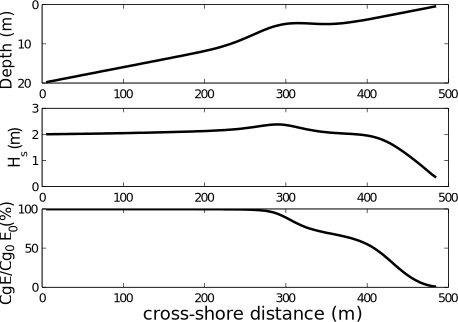
\includegraphics[width=0.6\textwidth]{FIGS_CH_SURF/surfer_en.pdf}}
%\vspace{3.64in}
  \caption{Evolution of significant wave height during breaking}
    {Results of the model by \cite{Thornton&Guza1986}  for a wave period $T=12$~s and 20$^\circ$ incidence angle 
    in 20~m depth. Waves propagate over a schematic beach with a mean slope $\beta=0.04$ 
    and a bar at $x=300$~m.}
\label{fig:surfer}
\end{figure}
%%%%%%%%%%%%% end of figure
Looking at the energy only, it is possible to have a good approximation of the 
evolution of the wave energy with a wave dissipation parameterized following the hydraulic jump model presented in chapter \ref{ch_sourceterms}. This was first 
developed in models for the total wave energy by \cite{Battjes&Janssen1978} and \cite{Thornton&Guza1983}. 
An example result from the model by Thornton and Guza, is shown in figure \ref{fig:surfer}. 

Although the wave height is a key parameter, the important application to sediment transport and beach morphodynamics requires 
more than information on energy only. First of all, orbital velocities at the bottom, which determine the re-suspension of 
sediments, require a knowledge of the wave spectrum, or at least wave periods. Hence these energy models have been 
extended in the form of wave action equations by defining suitable wave breaking parameterizations 
\citep[e.g.][]{Filipot&Ardhuin2012}. However, the spectral evolution also exhibits the development of harmonics 
and their progressive release over varying bathymetry. These processes 
and the reproduction of the important asymmetry of the waves requires an investigation of the relative phase of 
the wave components.
The relative phases of the different components are given by the 
bi-spectrum, which is defined as a generalization of the spectrum (our equation \ref{eq3.3}), 
\begin{equation}
B(\omega_i,\omega_j) = \langle a_{m,i} a_{m,j} a_{m,i+j} \rangle. 
\label{eq:bispecdef}
\end{equation}
This bi-spectrum is a complex number. Just like the spectrum is the Fourier transform of the 
2-point correlation function, the bi-spectrum  is the 2D Fourier transform of the 3-point correlation 
function of a time series, 
\begin{eqnarray}
S(\tau_1,\tau_2)&=& \langle \zeta(t) \zeta(t+\tau_1) \zeta(t+\tau_2)\rangle \\
B(\omega_1,\omega_2)&=& \frac{1}{(2 \pi)^2} \int_{-\infty}^\infty \int_{-\infty}^\infty S(\tau_1,\tau_2)
\mathrm{e}^{-\ir \omega_1 \tau_1  -\ir \omega_2 \tau_2 } \mathrm{d}\tau_1   \mathrm{d}\tau_2.
\end{eqnarray}
More properties of the bi-spectrum in the context of ocean waves are discussed in \cite{Hasselmann&al.1963}. 
We will particularly note that $B$ is zero for a Gaussian wave field. The skewness and asymmetry of the 
time series are given by integrals of the bi-spectrum, 
\begin{eqnarray}
 \langle  \zeta^3(t)\rangle &=& 12 \sum_n \sum_l \Re\left[ B(\omega_n,\omega_l)\right] + 6 \sum_n \Re\left[ B(\omega_n)\right] \\
\left\langle  \left(\frac{\partial \zeta}{\partial t}\right)^3 \right\rangle &=& 12 \sum_n \sum_l \Im\left[ B(\omega_n,\omega_l)\right] 
 + 6 \sum_n \Im\left[ B(\omega_n)\right]/ \left(\langle \zeta^2(t)\rangle\right)^{3/2},
\end{eqnarray}
where $\Re$ and $\Im$ stand for the real and imaginary parts respectively. 

For practical purposed the bi-spectrum is generally normalized to obtain a bi-coherence $b(\omega_1,\omega_2)$, with values between 0 and 1, 
and a bi-phase $\beta(\omega_1,\omega_2)$, 
\begin{eqnarray}
b(\omega_i,\omega_j)& =&\frac{\left|B(\omega_i,\omega_j)\right|}{\sqrt{ \left\langle  \left|a_{m,i} a_{m,j}\right|^2 \right\rangle 
                             \left\langle \left|a_{m,i+j}\right|^2   \right\rangle}}, \\
 \beta(\omega_i,\omega_j) &=&\arctan \left[\frac{\Im[     B(\omega_i,\omega_j)]}{\Re[     B(\omega_i,\omega_j)]} \right].
\end{eqnarray}
In the absence of phase-correlations between different components, $b=0$ and all waves are free and propagate at the linear phase speed.  
The other extreme are the harmonics of a monochromatic waves for which $b=1$. In that case the harmonics are bound to the underlying wave and propagate at its velocity, different from the linear phase speed. 

Real waves in shallow water are intermediate between these two extremes and harmonics are partially locked and can be released as free waves by changes in the bottom topography \citep[e.g.][]{Senechal&al.2003}.

\cite{Elgar&Guza1985b} have made one of the first analyses of the bi-spectral evolution on a gently sloping beach as part of the 
Nearshore Sediment Transport Study (NSTS) experiment. 
%%%%%%%%%%%%% figure
\begin{figure}[htb]
\centerline{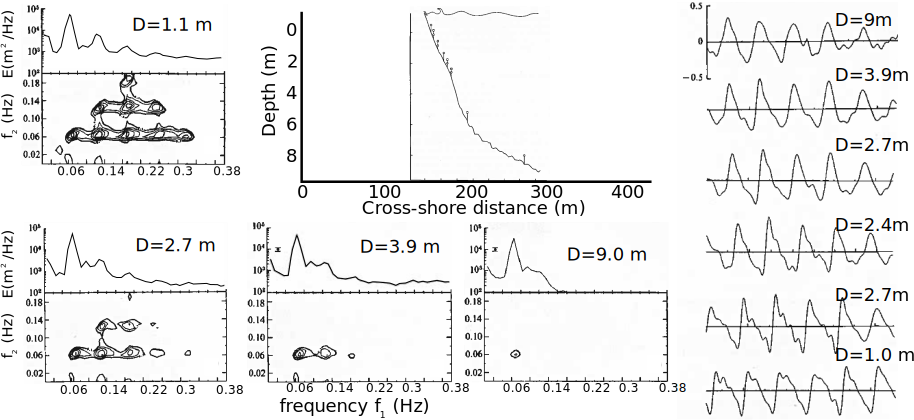
\includegraphics[width=\textwidth]{FIGS_CH_SURF/Elgar_Guza_spectra.pdf}}
%\vspace{3.64in}
  \caption{Spectral and bi-spectral evolution recorded on February 2, 1980.}
    {The position of bottom-mounted pressure gauges is shown  in  the upper-middle panel, from 9 m depth to 1.1 m depth. 
    Short pieces of the time series of surface elevation at the different sensors is shown in the right panel. 
    Left and bottom panels show spectra $E(f_1)$ and 
    and associated bi-coherence $b(f_1,f_2)$ at selected locations. Adapted 
    from \cite{Elgar&Guza1985b}.}
\label{fig:NSTS_bispectra}
\end{figure}
%%%%%%%%%%%%% end of figure
Figure \ref{fig:NSTS_bispectra} shows the evolution of time series of surface elevation, estimated from bottom-mounted pressure gauges, 
and the statistical representation of phase-relationships give by the bi-coherence. From a superposition of uncorrelated waves in 9~m depth, 
the spectrum evolves with the generation of harmonics that, on this particular beach, remain locked in phase and exchange energy. 
In 3.9~m depth, the bi-coherence already has 3 peaks at 0.06, 0.12 and 0.18~Hz that show the non-linear interaction of the main peak 
and its harmonics. In other cases with a more complex topography, \cite{Senechal&al.2003} showed the the harmonics can 
become free and the bi-coherence can be reduced after wave propagation over a bar. 

A representation of this 
effect as a  'triad' interactions  source term  in the wave action equation can be expressed theoretically 
from the bi-spectrum \citep{Herbers&Burton1997,Becq1998}. However, the integration of an evolution equation 
for the bi-spectrum comes at a considerable cost, although this is still much less than the cost of a phase-resolving models. 
As a result, most spectral wave models have adopted relatively crude parameterizations of the triad interactions
\citep[e.g.][]{Eldeberky&Battjes1995}. 


\section{Infragravity waves}\label{sec:IG}
\subsection{Observations}
 In the same way that sum interactions $f=f_1 + f_2$  give rise to harmonics, difference interactions 
 $f=f_1 - f_2$ also produce very low frequency components that are called infragravity waves, that we will often shorten as 'IG waves'. 
 This beating pattern was first 
 investigated by \cite{Munk1949}. Infragravity water level oscillations are often dominant in the swash, with a typical range of periods
 between 30~s (0.033~Hz) and 5~minutes (0.003~Hz). Figure \ref{fig:NSTS_IG} shows spectra of surface elevation from off-shore of the surf zone 
 to the swash zone, with a typical wind-sea spectrum transforming into a spectrum dominated by motions at frequencies below 0.04~Hz.
%%%%%%%%%%%%% figure
\begin{figure}[htb]
\centerline{\includegraphics[width=0.8\textwidth]{FIGS_CH_SURF/Elgar_Guza_spectra_IG.pdf}}
%\vspace{3.64in}
  \caption{Spectra of surface elevation recorded in Santa Barbara on February 4, 1980.}
    {Measurements at $D=0$~m were performed with a run-up wire: the elevation is not at a fixed position in $x$ but along the beach profile. Adapted 
    from \cite{Elgar&Guza1985b}.}
\label{fig:NSTS_IG}
\end{figure}
%%%%%%%%%%%%% end of figure
These long period oscillations of the water level are readily observed by video systems, as shown in figure \ref{fig:video_runup}. Their analysis 
is very important for the understanding of coastal hazards. 
 %%%%%%%%%%%%% figure
\begin{figure}[htb]
\centerline{\includegraphics[width=\textwidth]{FIGS_CH_SURF/runup_Stockdon.pdf}}
%\vspace{3.64in}
  \caption{Measurement of run-up using a video system}
    {Left: Snapshot of the beach at Duck, North Carolina, with the white line marking the position of a transect. Right: 
    time-stack of pixel grey values along this transect. The red line marks the detected edge of the water: using the beach profile $h(x)$ this 
    gives a time series of run-up. Adapted 
    from \cite{Stockdon&al.2006}.}
\label{fig:video_runup}
\end{figure}
%%%%%%%%%%%%% end of figure

The contribution of IG waves to the run-up is relatively larger for small beach slopes \citep{Stockdon&al.2006}, with some exceptions. 
The highest measured IG wave heights, around 2.5~m, was recorded on the cliff 
of the small island of Banneg, France, as shown in figure \ref{fig:NSTS_IG}. 
 %%%%%%%%%%%%% figure
\begin{figure}[htb]
\centerline{\includegraphics[width=\textwidth]{FIGS_CH_SURF/Banneg_IG.pdf}}
%\vspace{3.64in}
  \caption{Large infragravity wave heights measured on Banneg Island, France.}
    {Left: (a) Time series of pressure converted to surface elevation (assuming hydrostatic pressure) from the sensors at the top of the cliff (P2, red) and the bottom of the cliff (P3, blue). 
    A typical burst of high water levels, lasting 90~s, is enlarged in (b). Center: cliff profile and schematic of water level at the time
    of highest recorded pressure. Right, picture of the cliff from P3, at low tide. Adapted 
    from \cite{Sheremet&al.2014}.}
\label{fig:Banneg_IG}
\end{figure}
%%%%%%%%%%%%% end of figure


\subsection{Theories for IG waves generation}
A first theoretical explanation for the formation of infra-gravity waves was given by \cite{Witham1962} and \cite{Longuet-Higgins&Stewart1962},  looking 
at the flow response to the passage of wave groups. They actually gave two derivations, the first follows the perturbation method used in chapter \ref{ch1b}. The second method, which we will use here, is only applicable when wave groups are long compared to the water depth, 
and uses the wave-averaged mass and momentum equation, (\ref{Phillips_mom}) and (\ref{Phillips_mass}). 
Neglecting 
the Coriolis force, advection, and surface and bottom friction, these become, for waves propagating in the $x$ direction only 
\begin{eqnarray}
\frac{\partial M}{\partial t}&=& - \rho_w g D \frac{\partial \overline{\zeta}}{\partial x}  - \frac{\partial S_{xx}^{\mathrm{rad}}}{\partial x},  \\
\frac{\partial M}{\partial x}&=& - \rho_w  \frac{\partial  \overline{\zeta}}{\partial t}.
\end{eqnarray}

These are exactly the equation of long waves (i.e. in the shallow water limit),forced by $S_{xx}^{\mathrm{rad}}$. For a narrow wave spectrum, we note that
$S_{xx}^{\mathrm{rad}}$ is 
attached to the wave groups and travels at the speed $C_g$, the solution of such a forced wave is bound to travel with the forcing, so that  the time 
derivative is equal to $-C_g$ times the horizontal gradient. 

We recall eq. (\ref{eq:Sxx}) that gives $S_{xx}^{\mathrm{rad}}=\rho_w g E (2 C_g/C - 0.5)$, which is always positive. 
Taking a particular case of modulation of energy $E=E_0+ E_1 \cos [K x (1-C_g t)]$, we have
$S_{xx}^{\mathrm{rad}} = S_0 + S_1 \cos [K x (1-C_g t)]$ we look for solutions of the form, $M=M_1  \cos [K x (1-C_g t)]$
and  $\overline{\zeta}=A_1  \cos [K x (1-C_g t)$.  Replacing in our mass and momentum equation, this gives, 
\begin{eqnarray}
C_g M_1 &=& - \rho_w g D A_1 -  S_1 \\
 M_1 &=& - C_g \rho_w  A_1,
\end{eqnarray}
which gives the transport and elevation amplitudes of the bound long wave, 
\begin{eqnarray}
M_1 &=& - \frac{Cg S_1}{gD - C_g^2}\\
 A_1 &=& - \frac{ S_1}{\rho_w (gD - C_g^2)}.
\end{eqnarray}
This solution thus gives a total transport $M_1$ by the long and short waves that is partly compensating 
the modulation of the wave-induced transport $\rho_w C_g E_1/C$. Because the compensation is not exact, the net divergence 
of the flow is driving a change in  mean sea level, with a lower level where the wave energy $E_1$ is larger.
It should be noted that this bound wave response has a singularity in the limit of shallow water when $C_g \rightarrow \sqrt{gD}$, this is 
the limit into which the interaction of two short waves and the long wave becomes resonant. 
%%%%%%%%%%%%% figure
\begin{figure}[htb]
\centerline{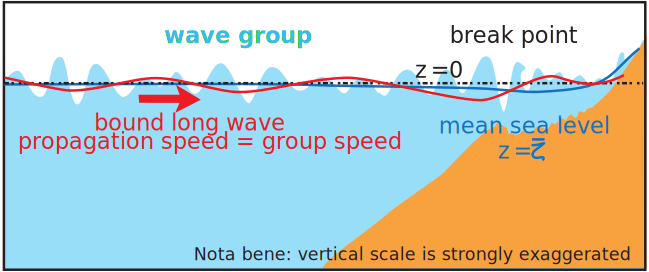
\includegraphics[width=0.6\textwidth]{FIGS_CH_SURF/Generation_IG_en.pdf}}
%\vspace{3.64in}
  \caption{Schematic of bound infragravity waves associated to wave groups.}
    \label{IGfig}
\end{figure}
%%%%%%%%%%%%% end of figure

This 180$^\circ$ phase shift between the wave energy and the long waves was indeed verified in some experiments, typically just outside the surf zone on 
gently sloping beaches, but it is typically less in the surf zone \citep{Elgar&Guza1985b}. This may be due to the difference between  the flat bottom 
solution where the long wave is exactly bound, and the real case of a varying depth in which the long wave is partially free. For a general wave 
spectrum with waves in all directions, the theoretical bound response is integral over all possible pairs of waves, %as detailed in chapter \ref{chnl2}, 
and the theory 
is well verified over a flat bottom \citep{Herbers&al.1994a}. The free and bound IG wave energy can be separated using a bi-spectral analysis  
\citep{Herbers&al.1994a}. Free IG energy usually dominates even in 8~m depth, and even more so in deeper water \citep{Herbers&al.1995}. 

It is also possible that other mechanisms generate long period oscillations. In particular, over coral reefs, the modulation of the position of the initial wave breaking with wave groups 
can produce mean sea level oscillations that are rather in phase with the wave groups \citep{Symonds&al.1982}. 

\subsection{Free wave radiation from the coast}
Whatever the details of the generating process, it is clear that bound waves traveling with the incoming wave groups are released and partially dissipated in the 
surf zone where the groups are dissipated. Because the phase speed of the released waves is much larger than that of the incident waves, 
most of the energy is strongly trapped by refraction along the coast. 

Observations compiled by \cite{Ardhuin&al.2014} suggest that the free IG wave spectrum near the coast can be parameterized as, 
\begin{eqnarray}
 A_{IG} & =&    H_s T_{m0,-2}^2\label{eq:fit0} \\
{E}_{IG}(f)& = & 1.2 \alpha_1^2 \frac{k g^2}{C_g 2 \pi f} \frac{(A_{IG}/4)^2}{\Delta_f}   \left[\min( 1., 0.015\mathrm{Hz}/ f)\right]^{1.5} \label{eq:fit1} \\
{E}_{IG}(f,\theta) & = & {E}_{IG}(f) / (2 \pi ),
\label{eq:fit2} 
\end{eqnarray}
where $\alpha_1=6 \times 10^{-4}$~s$^{-1}$ might vary with bottom topography, and $\Delta_f = 0.0279$~Hz. 
The $k/C_g$ factor accounts for the shoaling of a broad directional spectrum, while the frequency shape of the spectrum
is given by the other terms. In the shallow water limit, i.e. $k D$ going to zero, this spectrum is constant up to $f=15$~mHz and 
decreases like $f^{-1.5}$ for higher frequencies. In that frequency range, this asymptote is identical to the form $\tanh(kD)^{-1.5}$ given by 
\cite{Godin&al.2013}. The differences at lower frequencies may be due to the fact that, in particular for $f < 2$~mHz, the measured wave 
field in the open ocean is mostly driven by atmospheric pressure and not IG waves radiated from shorelines \citep{Filloux1980,deJong&al.2003}.

Eq. (\ref{eq:fit2}) gives an estimate $\widehat{H}_{IG}$ of the infragravity wave height, 
\begin{equation}
H_{IG}   =  4 \sqrt{\int_{0.05~\mathrm{mHz}}^{30~\mathrm{mHz}} \widehat{E}_{IG}(f)\mathrm{d} f}.  \label{eq:fit3}  
\end{equation}



%A global model with such a source of free infragravity waves at the coast gives average IG wave heights shown in figure \ref{fig:IG_global}.
 %%%%%%%%%%%%% figure
%\begin{figure}[htb]
%\centerline{\includegraphics[width=0.7\textwidth]{FIGS_CH_SURF/IG_climatology.pdf}}
%\vspace{3.64in}
%  \caption{Mean values of $H_{IG}$ over (a) January and February 2008, (b) June and July 2008. 
%Small squares with numbers correspond to the location of DART stations 
%used for model validation. Taken from \cite{Ardhuin&al.2014}. \label{fig:IG_map}}
%\label{fig:IG_global}
%\end{figure}
%%%%%%%%%%%%% end of figure


%The reflected direction 
